\section {Visión general}
En esta sección se trata todos los aspectos relativos a la gestión del proyecto. Esta
pretende dar alcance a la meta del proyecto y los objetivos del mismo dentro de las
limitaciones dadas: alcance, tiempo, calidad y presupuesto. 

La gestión del proyecto comprende la implantación de una metodología de desarrollo, viéndose 
esta como la implantación de una serie de pasos, técnicas, procedimientos y demás recursos que
ayuden a desarrollar el producto software dentro de un marco de trabajo. 

Por otro lado también se ha de tratar la planificación del proyecto, quedando este organizado en una 
serie de tareas y actividades derivadas de la metodología implantada. 

En la ejecución de un proyecto es necesario la inversión de una serie de recursos, tales como herramientas, 
personal, equipos, herraminetas... Se ha de determinar los recursos asignados a la ejecución del mismo, así como los roles 
de las personas asignadas y la relación entre estas.

El desarrollo de un proyecto software tiene unos costes derivados de los recursos asociados al mismo. Estos recursos
serán tanto materiales como humanos, y tendrán un coste fijo asociado que se utilizará para el cálculo del coste total.

Otra de las tareas que se llevan a cabo durante la gestión de un proyecto software es el análisis de riesgos. Todo proyecto 
esta sujeto a una probabilidad de que se den escenarios de riesgo en los que se pueda ver perjudicada la correcta realización del mismo. 
Se detectarán, listarán y analizarán los riesgos y sus consecuencias, así como la probabilidad de que estos sucedan y las prácticas que se llevarán 
a cabo para mitigar los efectos derivados de estos.

Por útltimo se expondrán las prácticas seguidas para asegurar la calidad del desarrollo y los productos obtenidos en cada paso de la
metodología. Para ello se incuyen estándares seguidos los estándares, prácticas y normas aplicables durante el desarrollo. Además 
se recogen los distintos tipos de revisiones,verificaciones y validaciones que se han llevado a cabo, así como los criterios 
para la aceptación o rechazo de cada producto y los procedimientos para implantar acciones correctoras o preventivas.

La planificación expuesta no recoje aspectos como la instalación, el mantenimiento o el soporte. Esta se centra únicamente en el ciclo de desarrollo
del proyecto y no en los procesos posteriores, los cuales, aunque también forman parte del ciclo de vida hábil del software, no se encuentran dentro de 
las etapas de desarrollo del mismo.

\section{Metodología de desarrollo}

Para la realización del proyecto se ha seguido una metodología iterativa e incremental. Más concretamente se ha tomado como
base el proceso unificado de desarrollo de software, el cual sigue un enfoque diriguido por casos de uso y centrado en 
la arquitectura. 

El ciclo de vida sigue un enfoque en espiral, dividido en cuatro etapas: determinar objetivos, análisis de riesgos, desarrollo y planificación.

\begin{description}
\item[Determinar objetivos]: 
   \begin {itemize}
   \item Se fijan los productos a obtener: requisitos, especificación, manuales ...
   \item Se fijan las restrinciones a las que estará sujeta el proyecto
   \item Sólo en la primera iteración se lleva a cabo una planificación inicial en esta etapa.
   \end{itemize}
\item[Análisis de riesgos]: 
   \begin {itemize}
   \item Se estudia las posibles amenazas y eventos no deseados, así como los daños y consecuencias derivados de estos.
   \item Se evaluan las distintas alternativas que permitan minimizar los riesgos.
   \end{itemize}
\item[Desarrollo]: 
   \begin {itemize}
   \item Se lleva a cabo el desarrollo de lo fijado en las etapas anteriores.
   \item El desarrollo de cada iteración se divide en cuatro etapas: analisis, diseño, codificación y pruebas.
   \end{itemize}
\item[Planificación]:
   \begin {itemize}
   \item Se analiza los productos obtenidos y el estado del proyecto.
   \item Se lleva a cabo una planificación de la siguiente iteración del ciclo de vida.
   \end{itemize}
\end{description}

En un enfoque en espiral lo más común es que en la primera iteración se ofrezca un proptotipo del producto a desarrollar, 
no obstante en el proyecto abordado no ha sido así. En lugar de ello se ha planteado una primera iteración que recoja el alcance 
del proyecto, así como los requisitos y análisis de los riesgos globales, además se realiza una planificación de las iteraciones que seguirán. 
Las demás iteraciones contemplan un subconjunto de estos requisitos añandiéndose así en cada iteración características al software y afinando el 
análisis global llevado en la primera y siguientes iteraciones.

Para la realización de los productos obtenidos en cada paso de la metodología se a utilizado el lenguaje de modelado UML. 
\section{Planificación}

La planificación se divide en una serie de iteraciones. Todas las 
iteraciones con excepción de la primera tienen las mismas etapas
en función de la metodología seguida.

Las etapas y subetapas en las que se divide cada iteración son:

\begin {itemize}
\item Objetivos
\item Riesgos
\item Desarrollo
\begin{itemize}
\item Análisis
\item Diseño
\item Codificación
\item Pruebas
\end{itemize}
\item Planificación
\end {itemize}

La planificación tiene como punto de partida el día 03/11/2014, día en la que se 
comenzó el desarrollo del proyecto. Se ha tomado una jornada laboral de 8 horas, 
y una semana hábil de 5 días.

En cada etapa de la planificación se hacen labores de documentación para que
toda la información relativa al proyecto quede reflejada en la memoria 
del mismo. 

La primera etapa refleja un planteamiento general del proyecto, este se ha ido refinando 
con cada iteración del ciclo de vida. Para ello se han modificado los documentos obtenidos de 
iteraciones anteriores.

\subsection{General}
\begin{center}
\begin{figure}[h]
\centering
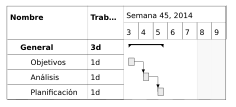
\includegraphics[scale=1]{planning/general.png} \\
\caption{General: 03/11/2014 - 05/11/2014 }
\end{figure}
\end{center}

\subsection{Expresiones lógicas}

\begin{center}
\begin{figure}[H]
\centering
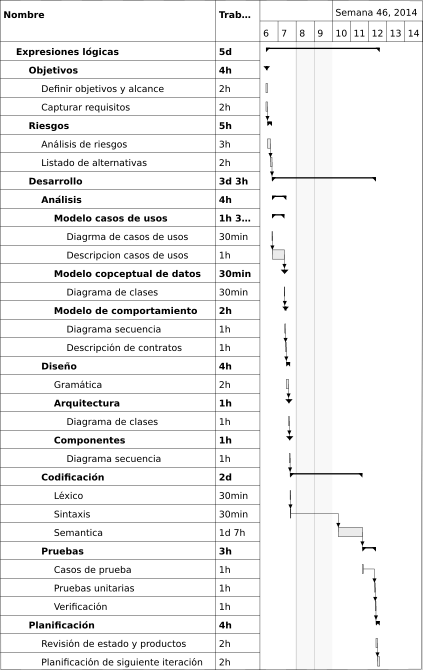
\includegraphics[scale=1]{planning/2-expresiones-logicas.png} \\
\caption{Exp. lógicas: 06/11/2014 - 12/11/2014 }
\end{figure}
\end{center}

\subsection{Sentencias de entrada/salida}

\begin{center}
\begin{figure}[H]
\centering
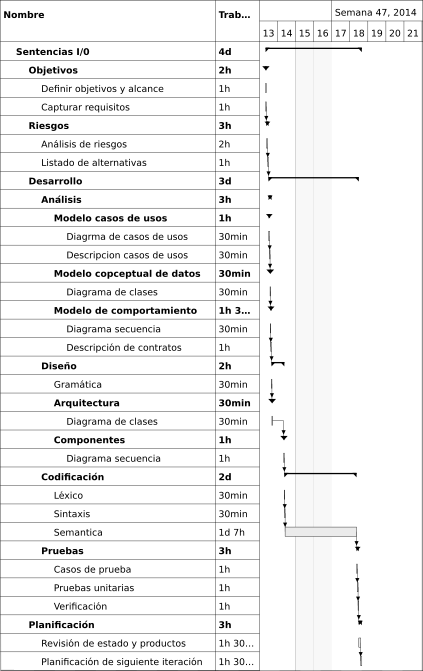
\includegraphics[scale=1]{planning/3-sentencias-io.png} \\
\caption{Sentencias I/O: 13/11/2014 - 18/11/2014 }
\end{figure}
\end{center}

\subsection{Sistema de errores}

\begin{center}
\begin{figure}[H]
\centering
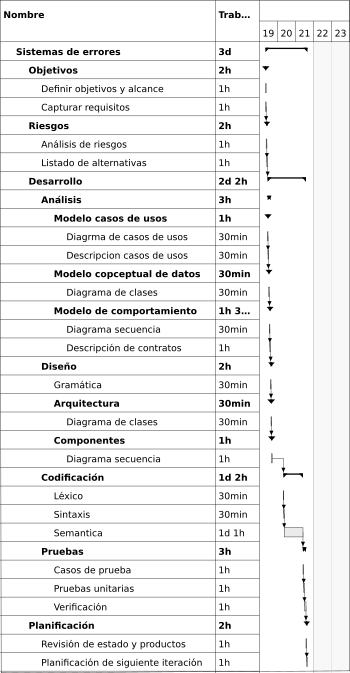
\includegraphics[scale=1]{planning/4-sistema-errores.png} \\
\caption{Sistema de errores: 19/11/2014 - 21/11/2014 }
\end{figure}
\end{center}

\subsection{Expresiones aritméticas}
\begin{center}
\begin{figure}[H]
\centering
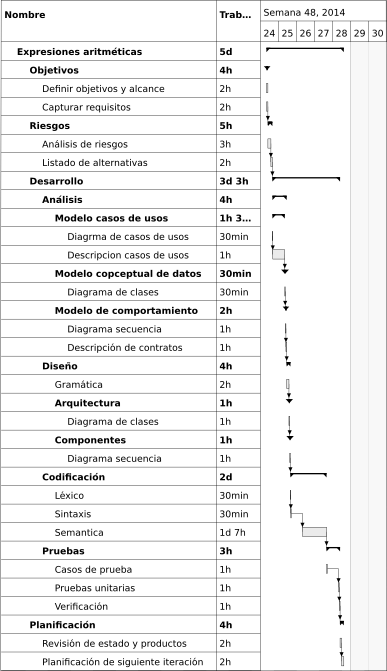
\includegraphics[scale=1]{planning/5-expresiones-aritmeticas.png} \\
\caption{Exp. aritméticas: 24/11/2014 - 28/11/2014 }
\end{figure}
\end{center}

\subsection{Símbolos variables}
\begin{center}
\begin{figure}[H]
\centering
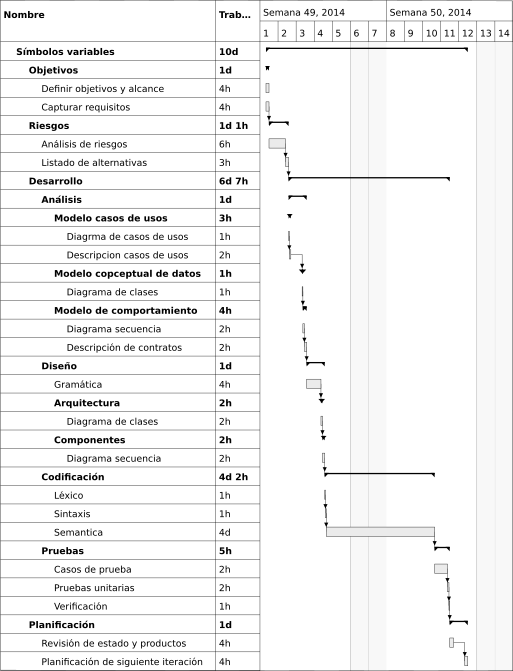
\includegraphics[scale=1]{planning/6-simbolos-variables.png} \\
\caption{Símbolos variables: 01/12/2014 - 14/12/2014 }
\end{figure}
\end{center}


\subsection{Sentencias de control I}
\begin{center}
\begin{figure}[H]
\centering
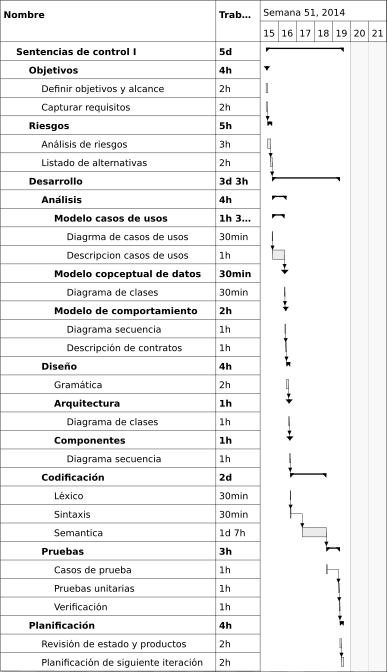
\includegraphics[scale=1]{planning/7-sentencias-control-i.png} \\
\caption{Sentencias control I: 15/12/2014 - 19/12/2014 }
\end{figure}
\end{center}

\subsection{Interfaz de usuario I}
\begin{center}
\begin{figure}[H]
\centering
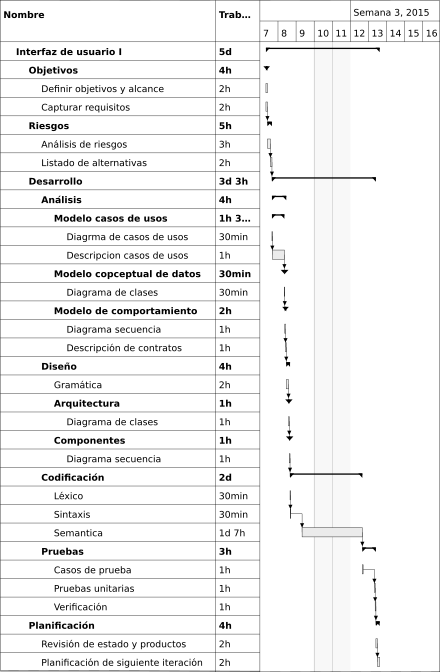
\includegraphics[scale=1]{planning/8-interfaz-usuario-i.png} \\
\caption{Interfaz usuario I: 07/01/2015 - 13/01/2015 }
\end{figure}
\end{center}


\subsection{Expresiones cadenas de caracteres}
\begin{center}
\begin{figure}[H]
\centering
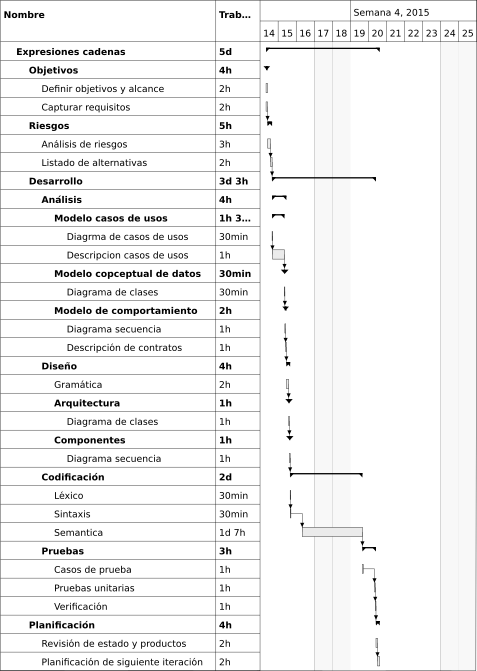
\includegraphics[scale=1]{planning/9-expresiones-cadenas.png} \\
\caption{Interfaz usuario I: 14/01/2015 - 20/01/2015 }
\end{figure}
\end{center}

\subsection{Conversión de tipos}
\begin{center}
\begin{figure}[H]
\centering
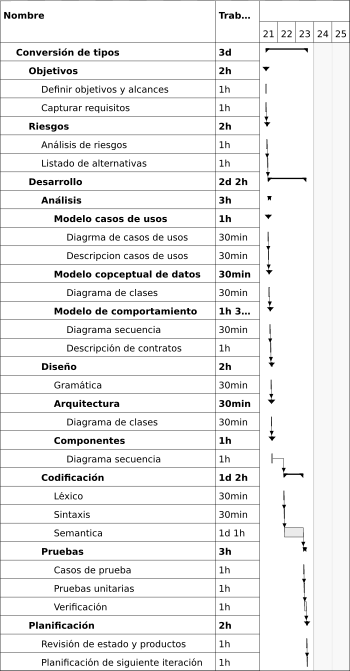
\includegraphics[scale=1]{planning/10-conversion-tipos.png} \\
\caption{Conversión de tipos: 21/01/2015 - 23/01/2015 }
\end{figure}
\end{center}


\subsection{Funciones de cadenas}
\begin{center}
\begin{figure}[H]
\centering
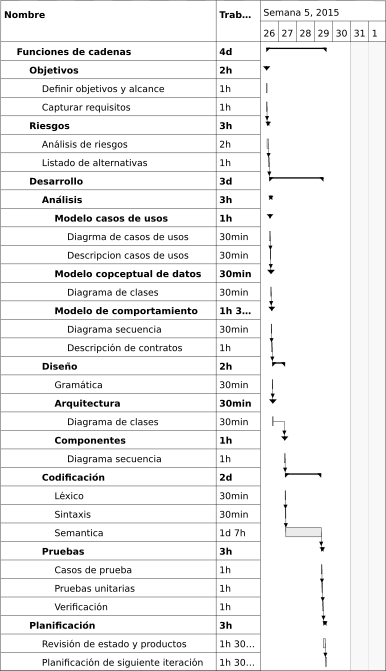
\includegraphics[scale=1]{planning/11-funciones-cadenas.png} \\
\caption{Funciones de cadenas: 26/01/2015 - 29/01/2015 }
\end{figure}
\end{center}

\subsection{Expresiones array}
\begin{center}
\begin{figure}[H]
\centering
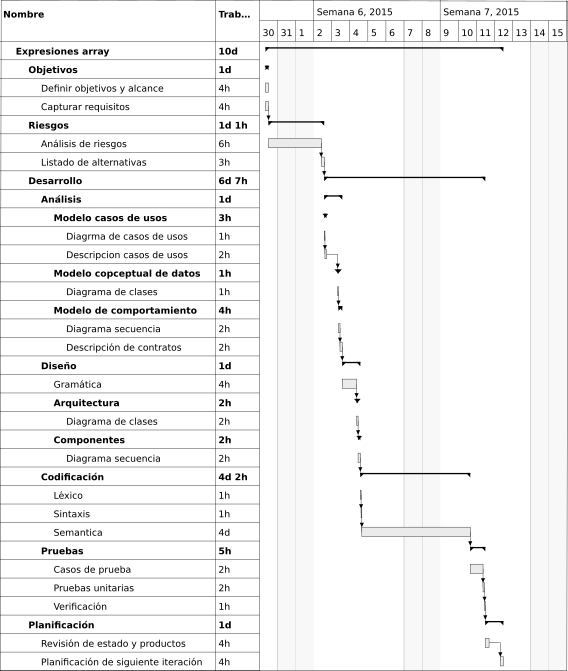
\includegraphics[scale=1]{planning/12-expresiones-array.png} \\
\caption{Expresiones array: 30/01/2015 - 12/02/2015 }
\end{figure}
\end{center}

\subsection{Símbolos funciones}
\begin{center}
\begin{figure}[H]
\centering
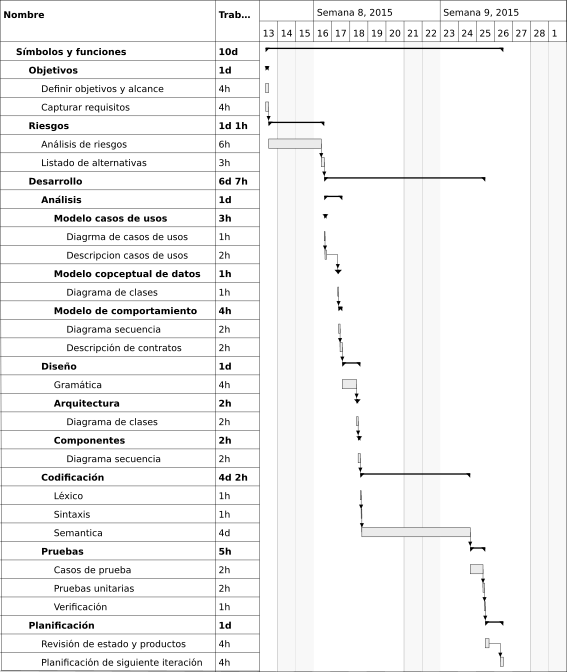
\includegraphics[scale=1]{planning/13-simbolos-funciones.png} \\
\caption{Símbolos funciones: 13/02/2015 - 26/02/2015 }
\end{figure}
\end{center}

\subsection{Expresiones regulares}
\begin{center}
\begin{figure}[H]
\centering
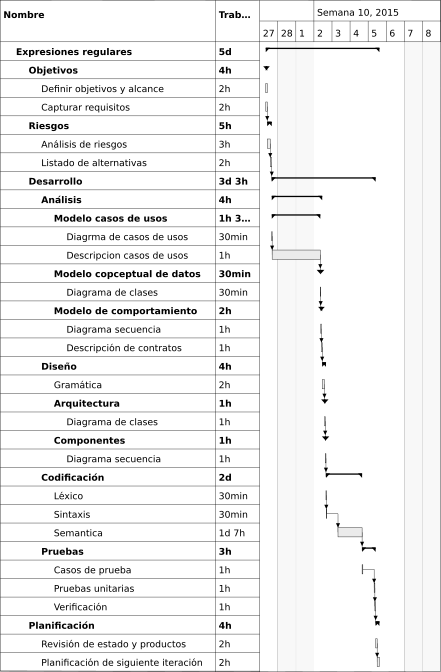
\includegraphics[scale=1]{planning/14-expresiones-regulares.png} \\
\caption{Expresiones regulares: 27/02/2015 - 05/03/2015 }
\end{figure}
\end{center}

\subsection{Símbolos clases I}
\begin{center}
\begin{figure}[H]
\centering
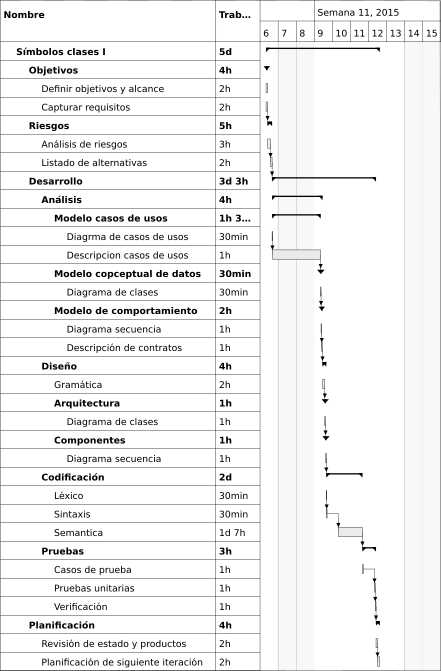
\includegraphics[scale=1]{planning/15-simbolos-clases-i.png} \\
\caption{Símbolos clases I: 06/03/2015 - 12/03/2015 }
\end{figure}
\end{center}


\subsection{Expresiones condicionales}
\begin{center}
\begin{figure}[H]
\centering
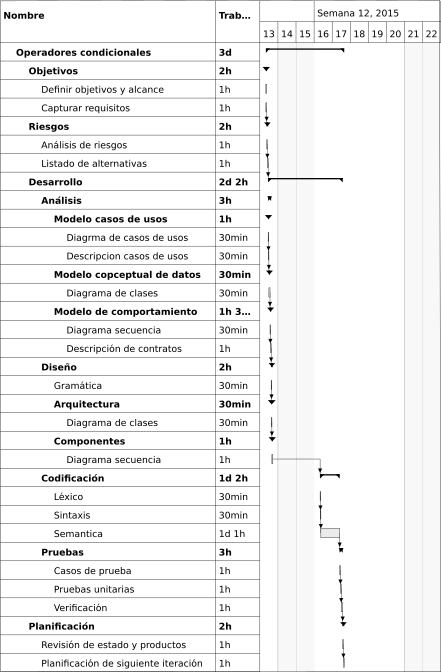
\includegraphics[scale=1]{planning/16-expresiones-condicionales.png} \\
\caption{Expresiones condicionales: 13/03/2015 - 17/03/2015 }
\end{figure}
\end{center}

\subsection{Funciones de depuración}
\begin{center}
\begin{figure}[H]
\centering
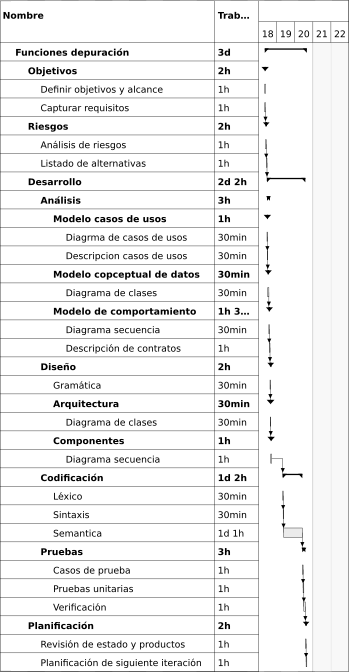
\includegraphics[scale=1]{planning/17-funciones-depuracion.png} \\
\caption{Fúnciones de depuración: 18/03/2015 - 20/03/2015 }
\end{figure}
\end{center}


\subsection{Optimización de memoria}
\begin{center}
\begin{figure}[H]
\centering
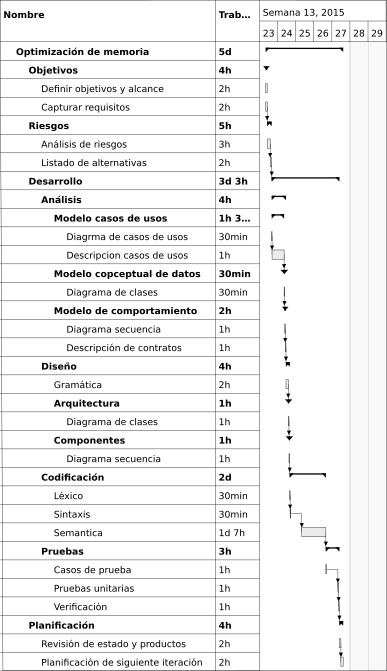
\includegraphics[scale=1]{planning/18-optimizacion-memoria.png} \\
\caption{Optimización de memoria: 23/03/2015 - 27/03/2015 }
\end{figure}
\end{center}

\subsection{Sentencias de control II}
\begin{center}
\begin{figure}[H]
\centering
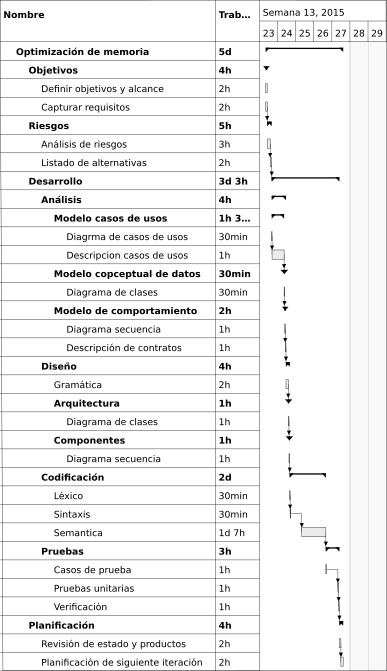
\includegraphics[scale=1]{planning/18-optimizacion-memoria.png} \\
\caption{Optimización de memoria: 23/03/2015 - 27/03/2015 }
\end{figure}
\end{center}


\subsection{Paso de argumentos}
\begin{center}
\begin{figure}[H]
\centering
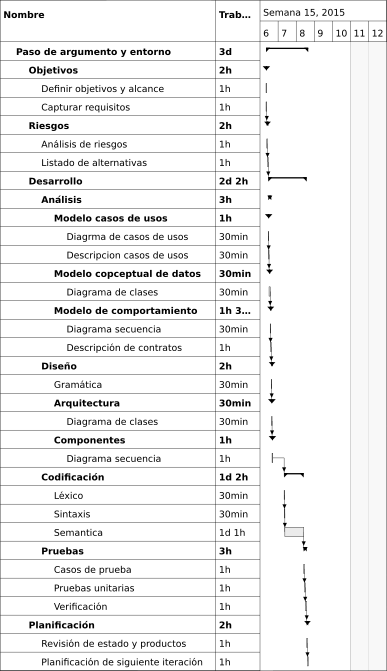
\includegraphics[scale=1]{planning/20-paso-argumentos.png} \\
\caption{Paso de argumentos: 06/04/2015 - 08/04/2015 }
\end{figure}
\end{center}

\subsection{Interfaz de usuario II}
\begin{center}
\begin{figure}[H]
\centering
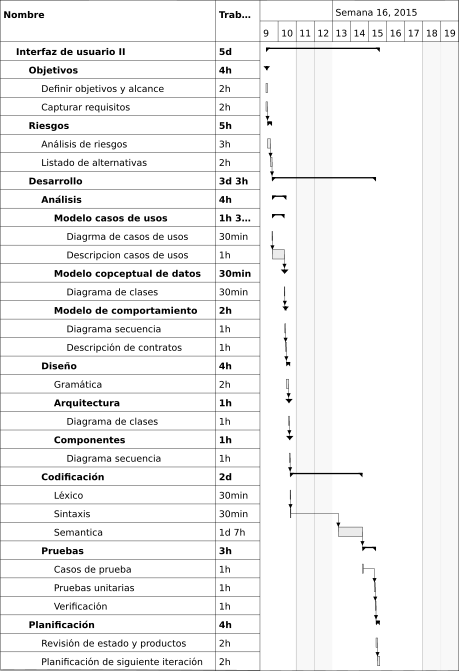
\includegraphics[scale=1]{planning/21-interfaz-usuario-ii.png} \\
\caption{Interfaz de usuario II: 09/04/2015 - 15/04/2015 }
\end{figure}
\end{center}

\subsection{Procesos I}
\begin{center}
\begin{figure}[H]
\centering
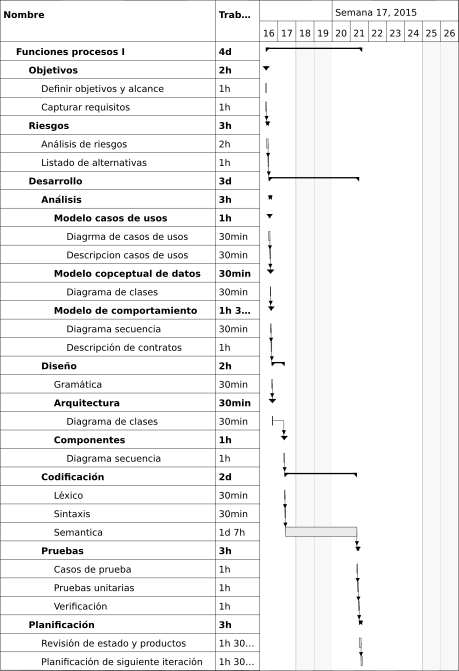
\includegraphics[scale=1]{planning/22-funciones-procesos-i.png} \\
\caption{Procesos I: 16/04/2015 - 21/04/2015 }
\end{figure}
\end{center}

\subsection{Fechas y tiempo}
\begin{center}
\begin{figure}[H]
\centering
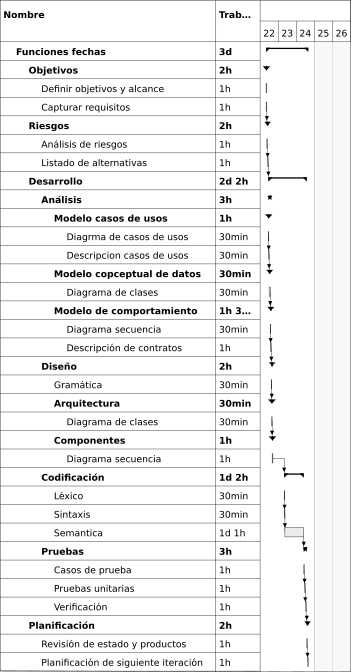
\includegraphics[scale=1]{planning/23-funciones-fechas.png} \\
\caption{Fechas y tiempo: 22/04/2015 - 24/04/2015 }
\end{figure}
\end{center}

\subsection{Ficheros}
\begin{center}
\begin{figure}[H]
\centering
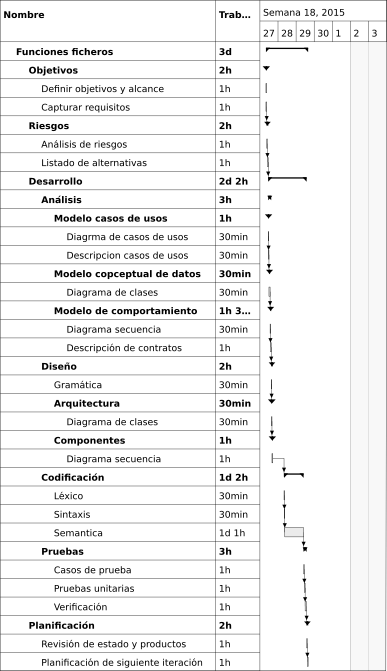
\includegraphics[scale=1]{planning/24-funciones-ficheros.png} \\
\caption{Ficheros: 27/04/2015 - 29/04/2015 }
\end{figure}
\end{center}

\subsection{Extensiones}
\begin{center}
\begin{figure}[H]
\centering
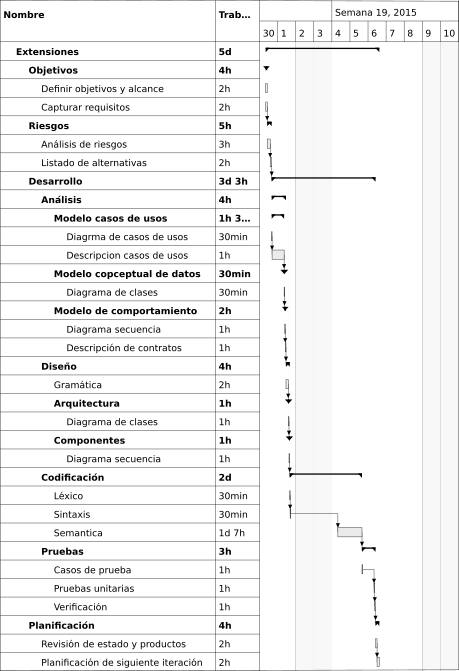
\includegraphics[scale=1]{planning/25-extensiones.png} \\
\caption{Extensiones: 30/04/2015 - 06/05/2015 }
\end{figure}
\end{center}

\subsection{Extensión gettext}
\begin{center}
\begin{figure}[H]
\centering
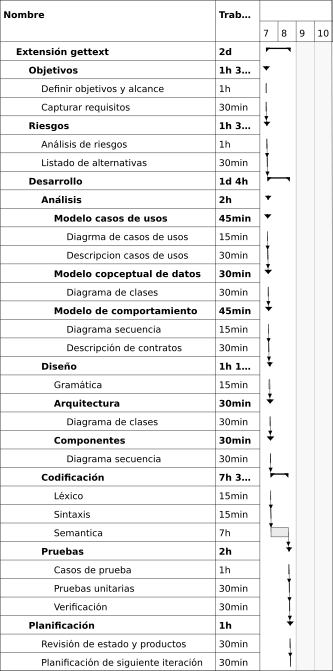
\includegraphics[scale=1]{planning/26-extension-gettext.png} \\
\caption{Extensiones gettext: 07/05/2015 - 08/05/2015 }
\end{figure}
\end{center}


\subsection{Procesos II}
\begin{center}
\begin{figure}[H]
\centering
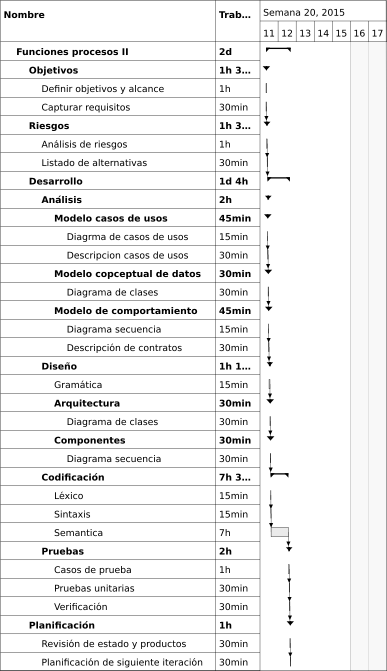
\includegraphics[scale=1]{planning/27-funciones-procesos-ii.png} \\
\caption{Procesos II: 11/05/2015 - 12/05/2015 }
\end{figure}
\end{center}

\subsection{Símbolos clases II}
\begin{center}
\begin{figure}[H]
\centering
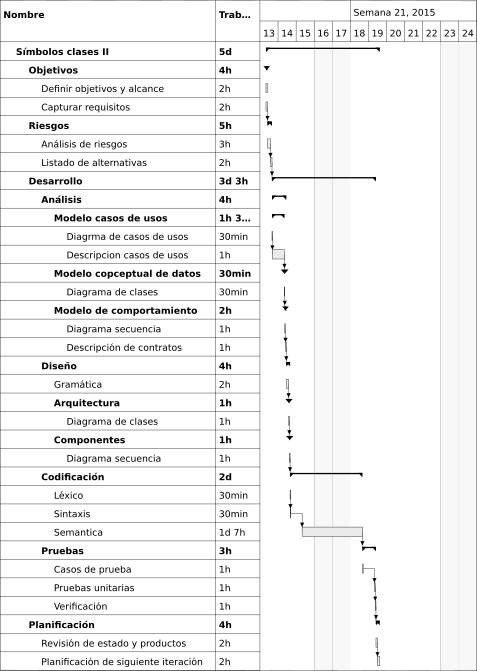
\includegraphics[scale=1]{planning/28-simbolos-clases-ii.png} \\
\caption{Símbolos clases II: 13/05/2015 - 19/05/2015 }
\end{figure}
\end{center}



\subsection{Símbolos funciones II}
\begin{center}
\begin{figure}[H]
\centering
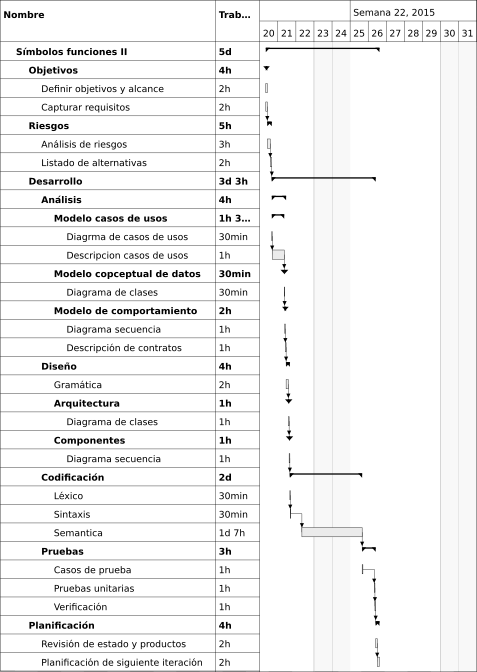
\includegraphics[scale=1]{planning/29-simbolos-funciones-ii.png} \\
\caption{Símbolos funciones II: 20/05/2015 - 26/05/2015 }
\end{figure}
\end{center}

\subsection{Extensión mysql}
\begin{center}
\begin{figure}[H]
\centering
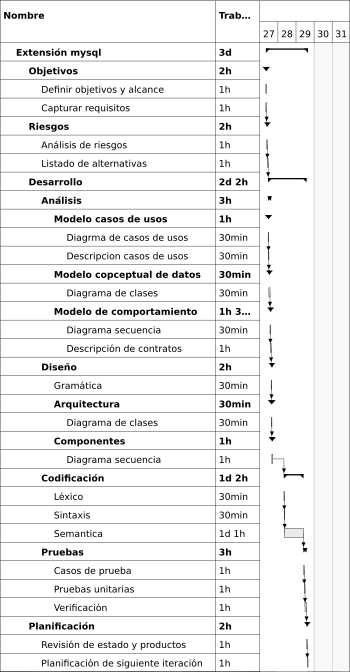
\includegraphics[scale=1]{planning/30-extension-mysql.png} \\
\caption{Extensión mysql: 27/05/2015 - 29/05/2015 }
\end{figure}
\end{center}





\section{Organización}
Para la realización del proyecto se ha utilizado los siguientes recursos humanos :
\begin{description}
\item[Empleado 1:] Director de proyecto, control de calidad. 
\item[Empleado 2:] Analista, diseñador de arquitectura, diseñador de sistemas, desarrollador, tester.
\end{description}

Además se han utilizado los siguientes recursos materiles:
\begin{description}
\item [Equipo de trabajo 1:] Computadora para las tareas de gestión y administración. 
\item [Equipo de trabajo 2:] Computadora para las tareas de desarrollo y documentación
\end{description}

Las herraminetas utilizas son las siguientes:
\begin{description}
\item [Sistema operativo:] GNU/Linux. 
\item [Entorno integrado de desarrollo:] Geany.
\item [Generador léxico:] Flex.
\item [Generador sintáctico:] Bison.
\item [Compilador:] GCC.
\item [Depurador:] GDB.
\item [Herramientas para la construcción automática:] Autoconf, automake, make.
\item [Desarrollo de diagramas:] Dia, railroad diagram generator.
\item [Control de versiones:] Subversion.
\item [Creación de documentación:] Latex.
\item [Planificación:] Planner.
\item [Bibliotecas de desarrollo:] readline, boost. 
\item [Comunicación:] Servicio gratuito de correo electrónico. 
\end{description}

\section{Costes}
A continuación se presenta el coste relativo a los recursos humanos invertidos en el desarrollo del 
proyecto. Para ello se ha tomado como referencia el documento BOE publicado el sábado 30 de nobiembre de 2013
por el ministerio de empleo y seguridad social. En este documento se recoje la tabla salarial según
el convenio colectivo de la empresa Trevenque Sistemas de Información SL.

\begin{tabular}{|l|l|l|l|} \hline
\textbf{Empleado} & \textbf{Grupo} & \textbf{Salario anual bruto} & \textbf{Salario mensual bruto}  \\ \hline
Empleado 1 & Directivo técnico & 26.652,92€ & 2.221,07€  \\ \hline
Empleado 2 & Programado senior & 18.120,00€ & 1.510,00€ \\ \hline
\end{tabular}

El tiempo de desarrollo asciende a 8 meses. El coste de los recursos humanos es:

\begin{tabular}{|l|l|} \hline
\textbf{Empleado 1} &  17.768,56€ \\ \hline
\textbf{Empleado 2} &  12.080,00€ \\ \hline
\textbf{Total} &  29.848,56€ \\ \hline
\end{tabular}
 
 Para el desarrollo del proyecto se ha necesitado de dos equipos con una potencia y prestaciones medias. El
 coste de los recursos materiales que suponen estas computadores es:
 
 \begin{tabular}{|l|l|l|} \hline
\textbf{Computador \tiny{i5-4460/ 4GB/ 1TB} } & 2x & 409,00€ \\ \hline
\textbf{Total} & & 818,00€ \\ \hline
\end{tabular}

Las herramientas utilizadas en el desarrollo del proyecto tiene licencia libre. El uso de estas herramientas no
suponen coste adicional para el desarrollo del proyecto. 

\section{Riesgos}

En este punto se muestran listan los riesgos identificados. Estos pueden originar un efecto negativo en el 
desarrollo del proyecto. Además se muestra la probabilidad de que estos se den y el impacto que tendrían. 
Una vez identificados los riesgos se definen los planes seguidos para reducir los efectos derivados estos o disminuir
la probabilidad de que ocurran.

El análisis de riesgos se ha llevado a cabo en cada iteración del ciclo de desarrollo. Cada iteración a completado la 
información mostrada. Muchos de los riesgos indicados son comunes a todas las iteraciones realizadas. 

Los riesgos analizados según el impacto que pueden ocasionar en el proyecto quedan divididos en:
\begin {description}
\item[Insignificantes:] No merecen ser tenido en cuenta.
\item[Tolerables:] Están dentro de un marge de aceptación, por tanto no compromenten ni el proyecto, ni el producto ni la organización.
\item[Graves:] Compromente gravemente el proyecto, el producto o la organización.
\item[Críticos:] Amenaza la supervivencia del proyecto o el producto o la organización.
\end{description}

Para dar claridad al análisis, la probabilidad de que se dé un determinado escenario de riesgo se presenta de forma relativa de la 
siguiente forma:
\begin{description}
\item[Muy baja:] $<10\%$.
\item[Baja:] del $10$ al $25\%$.
\item[Moderada:] del $25$ al $50\%$.
\item[Alta:] del $50$ al $75\%$.
\item[Muy alta:] $>75\%$.
\end{description}

Los riesgos quedan organizados en distintas categorías para un mejor análisis.

%~ Riesgos tecnológicos: derivados del software y hardware utilizados.
%~ Riesgos personales: asociados a las personas involucradas en el desarrollo.
%~ Riesgos organizacionales: relacionados a la organización.
%~ Riesgos de herramientas: resultantes de las herramientas de software utilizadas.
%~ Riesgos de requerimientos: surgen de los cambios en los requerimientos.
%~ Riesgos de estimación: proceden de las estimaciones de costes y recursos. 

\subsection{Riesgos tecnológicos}
Son los riesgos derivados del software y hardware necesarios para el desarrollo del 
proyecto.

\begin{tabular}{|l|c|c|} \hline
\textbf{Riesgo} & \textbf{Probabilidad} & \textbf{Impacto} \\ \hline
Los recursos no están disponibles a tiempo & Baja & Tolerable \\ \hline
\shortstack[l]{\\Fallos en el sistema operativo \\u otros software de sistema}  & Baja & Tolerable \\ \hline
Fallos en el hardware de desarrollo & Baja & Grave \\ \hline
Errores de configuración & Baja & Tolerable \\ \hline
\shortstack[l]{\\Actualización del sistema\\no realizada correctamente} & Baja & Tolerable \\ \hline
Integridad y privacidad de los datos & Baja & Grave \\ \hline
Manipulación deliberada de los programa & Moderada & Grave \\ \hline
\shortstack[l]{\\Las herramientas de comunicación \\ no se encuentran disponibles} & Baja & Insignificante \\ \hline
\shortstack[l]{\\El repositorio de código no se encuentra \\ disponible} & Baja & Tolerable \\ \hline
\end{tabular}

En el caso de que los recursos materiales, hardware de desarrollo, no estén disponibles a tiempo se puede comenzar con tareas de definición y 
análisis. Si la demora se hace demasiado extensa se cancelará el pedido del hardware y se realizará a otro proveedor. Esto puede ocasionar
un retraso de días que puede ser mitigado dedicando este tiempo a tareas en las que no se precise de hardware. 

Si se produce algún fallo en el software de sistema que da soporte al desarrollo este puede derivar en pérdidas de datos. La solución sería gestionar la incidencia
o reinstalar el sistema. La perdida de datos se puede mitigar si se realizan copias de seguridad periódicas. Como medida preventiva se pueden guardar puntos de restauración del sistema
para preveenir o mitigar la demora de tiempo que esto podría ocasionar.

Es posible que se produzcan fallos en el hardware sobre el cual se desarrolla el proyecto, esto puede ocasionar retrasos de entregas o la perdida de los datos. 
Para prevenir y mitigar este efecto negativo se puede realizar copias periódicas de los datos y mantener los equipos en un estado de funcionamiento óptimo, bien refigerados 
y sin exposición a agentes externos. 

Si se produce algún error en la configuración del sistema es posible que algunas características de este dejen de funcionar, en muchos casos esto puede llegar a ser perjudicial para 
el proyecto. Para prevenir y mitigar este efecto se deberán realizar copias de seguridad, además se deberá minizar la cantidad de software instalado en los equipos. En el caso de producirse un 
fallo de configuración del sistema que afecte directamente a la ejecución del proyecto se deberá invertir tiempo para corregir las causas y administrar el sistema.

En algunos casos una actualización del sistema que da soporte a la ejecución del proyecto puede ocasionar fallos en el mismo o en la configuración. Para ello además de 
las soluciones y practicas comentadas en los puntos anteriores, se puede minimizar el número de actualizaciones que no sean críticas o que no sean indespensables para 
el desarrollo del proyecto. Como medida de actuación el sistema deberá ser restablecido mediante un administrador cualificado. 

La integridad y privacidad de los datos se puede ver comprometida por algún uso indebido de los mismos o por agentes ajenos al proyecto. Para prevenir y mitigar los efectos de este escenario 
se realizarán copias de seguridad  periódicas y se hará uso de un software de control de versiones. Además se protegerá el acceso a los datos mediante técnicas como claves de acceso, configuraciones de red pocos permisivas
(por ejemplo mediante el uso de firewalls), configuraciones óptimas del sistema (en cuanto servicios y programas), cifrado, no permitir la conexión de dispositivos extraibles, etc. Es muy importante en este punto 
controlar además los permisos de publicación, transferencia y portabilidad que tienen los empleados sobre los datos, quedando registrada y validada toda operación de esta naturaleza. Como medida de
actuación ante un escenario de este tipo los datos quedarán en cuarentena y se llevará a acabo un análisis forense que determine los agentes implicados y los motivos.

Es posible que en algunos casos los programas que conforman el sistema sobre el que se desarrolla sean manipulado de forma consicinete o inconsiente por una persona integrante del equipo o ajena 
al mismo. Para prevenir este escenario se acotará el uso del equipo al propósito que este tiene, no se permitirá la instalación de software adicional, se protegerá el acceso al sistema mediante claves robustas y se 
usará software antivirus. Como medida de actuación se bloqueará el acceso al proyecto a cualquier software que se tenga constancia de que se encuentre manipulado o infectado por alguna clase del 
malware, y el equipo implicado se podrá en cuarentena para evaluar el impacto de lo ocurrido.  

Las herramientas de comunicación son un elemento clave en el desarrollo de un proyecto. Depender de terceros para dar soporte al proyecto en este aspecto puede llegar a ser perjudicial. Para 
prevenir pérdidas en el servicio se puede usar clientes estables, fiables y consolidados en el mercado. Para mitigar la perdida de información que supondría una caída del servicio se puede hacer
copias de toda la información enviada por estos medios. Como medida de actuación, simpre y cuando sea necesario una comunicación, se utilizarán otros medios de comunicación como el teléfono. 

El repositorio en el cual se aloja el código fuente puede sufrir caídas en el servicio. Para mitigar y prevenir este tipo de incidencias se alojará el sistema de control de versiones en alguna
máquina de la infraestructura local al proyecto. Esto bloquea o dificulta el acceso remoto al código, lo cual tiene sus ventajas ya que disminuye el grado de exposición, pero hace que el acceso 
al código esté condicionado por un equipo local, y por la disponibilidad y visibilidad de este. 

\subsection{Riesgos personales}
En esta sección quedan registrados los riesgos asociados a las personas involucradas en el proyecto. 

\begin{tabular}{|l|c|c|} \hline
\textbf{Riesgo} & \textbf{Probabilidad} & \textbf{Impacto} \\ \hline
Cambios en el personal directivo & Baja & Crítico \\ \hline
Cambios en el personal ejecutivo & Baja & Grave \\ \hline
\end{tabular}

Los cambios en el equipo directivo de un proyecto pueden amenazar drásticamente la supervivencia y desarrollo de este. 
El nuevo personal no tiene porque compartir los mismos criterios que el anterior, y lo normal es que no conozca aspectos
internos del mismo. Un cambio directivo en el proyecto puede ocasionar remplanteamientos de cuestiones que ya se encontraban cerradas.
Este tipo de riesgos es difícil de preveenir por otros medios que no sean contratos laborales, y aún así no se podría asegurar que el equipo se mantendrá. 
Para mitigar el efecto que un cambio de este tipo podría ocasionar toda decisión directiva deberá quedar analizada, argumentada y registrada. 

El personal ejecutivo es escencial para el desarrollo de un proyecto, por lo que un cambio de este tipo en el equipo puede suponer un alto riesgo 
para el desarrollo. Al igual que en el punto anterior los contratos laborales puden prevenir en cierto grado el riesgo. Para mitigar el efecto se 
deberá documentar todo los procesos y productos obtenidos. Como medida de actuación, siempre que sea posible, el anterior personal podría instruir al
nuevo hasta que tome la destreza y conocimientos suficientes.

\subsection{Riesgos organizativos}

En esta sección se presentan y analizan los riesgos relativos a la organización del proyecto. 

\begin{tabular}{|l|c|c|} \hline
\textbf{Riesgo} & \textbf{Probabilidad} & \textbf{Impacto} \\ \hline
Las tareas no quedan bien definidas y/o acotadas & Moderada & Tolerable \\ \hline
Las tareas no quedan bien distribuidas & Moderada & Tolerable \\ \hline
No se atribuyen responsabilidades & Baja & Tolerable \\ \hline
No se establece una jerarquía de prioridades & Baja & Tolerable \\ \hline
La comunciación entre el equipo no es suficente & Moderada & Tolerable \\ \hline
\end{tabular}

Si las tareas no quedan bien definidas y acotadas se originará fallos en la comunicación y el entendimiento entre
los integrantes del equipo, pudiendo en muchos casos originar trabajo extra y la consecuente dilatación en los tiempos. 
Para preveenir y mitigar este efecto se deberá realizar una descripción minusiosa y detallada de las mismas, utilizando un lenguaje 
sencillo y directo. El plan de actuación ante estas situaciones será la aclaración de los puntos que fueron confusos, mientras que la parte 
que no llegó a enteder las cuestiones planteadas no deberá presoponer y pidirá la aclaración pertinente. 

Si las tareas no se encuentran bien distribuidas puede darse esceso de trabajo por algunas de las partes, ocasionando efectos de parada en el 
proceso de desarrollo. Por otro lado otros recursos pueden quedar ociosos. Para evitar y mitigar este escenario se deberá analizar y planificar todo 
el trabajo a realizar. En el caso de que una planificación incorrecta derive en problemas de este tipo se deberá replantear el trabajo.

Un equipo en el que las responsabilidades no queden bien atribuidas puede originar en la falta de implicación y correción por alguna de 
las partes. Para prevenir y mitigar este efecto se deberá hacer una correcta planificación, incolucrando al personal y hacerles entender la imporancia de su trabajo. 

Si no se establece una jerarquía de prioridades en las tareas puede ocasionar la perdida de tiempo en tareas menos importantes, mientras que otras más prioritarias y de las que
existan dependencias quedarán paradas. 
Para evitar esto se deberá realziar una planificación y hacer entender a todo el equipo las prioridades marcadas. Bajo esta circustancias se deberá retribuir prioridades 
y hacer que todo el equipo sea consciente de estas.

Si no se mantiene una comunicación suficiente el proyecto puede verse perjudicado en su ejecución. El equipo directivo puede no conocer el estado verdadero del proyecto 
y las decisiones tomadas no contar con toda la información posible. Para mitigar y prevenir este escenario se pueden realizar reuniones constantes. Como medida de actuación ante 
esta situación se deberá comunicar a los implicados la importancia de la información que poseen.

\subsection{Riesgos de requisitos}

Son riesgos que surgen de los requisitos, ya sean debido a que estos han cambiado o que no se han recojido correctamente.

\begin{tabular}{|l|c|c|} \hline
\textbf{Riesgo} & \textbf{Probabilidad} & \textbf{Impacto} \\ \hline
Especificación de requisitos insuficiente & Moderada & Grave \\ \hline
Captura de requisitos errónea & Moderada & Grave \\ \hline
Casos de uso complejos o mal redactados & Baja & Tolerable \\ \hline
\shortstack[l]{\\No se han capturado todos los datos\\ que definen o con los que trabaja el sistema} & Baja & Tolerable \\ \hline
\shortstack[l]{\\Añadir nuevas características sin tener en\\ cuenta la arquitectura interna del sistema} & Alta & Tolerable \\ \hline
\end{tabular}

Si los requisitos no son enumerados y definidos de forma efectiva puede ocasionar un sistema que no hace lo que debe hacer. Para evitar esto 
se lleverá a cabo múltiples reuniones con el cliente para la toma de requisitos, donde el analista tomará parte activa de estas y nunca llegará a
presuponer ningún aspecto que no quede bien acotado. En este punto el analista podrá optar por algunas de las técnicas conocidas para la 
toma de requisitos. Como plan de actuación se deberá poner en conctacto con el cliente y pedir la aclaracón o especificación 
de los puntos que no quedaron fijados. 

De igual forma unos requisitos mal tomados puede tener como resultado un producto que no cumple con las espectativas. Para prevenir y evitar 
este escenario el analista debe ser muy conciso y minusioso en la toma de requisitos, haciendo que todo quede claro por ambas partes. 

Aunque se realice una toma de requisitos completa, queda la posibilidad que el analista no transmita correctamente qué va a hacer el sistema para dar solución a 
estos. Se deberá poner especial antención en que los casos de usos queden bien redactados, en un lenguaje simple y con la suficiente sencillez y completud. 

Una de las principales actividades de un sistema informaticos es procesar datos, dado que el valor de la información viene atribuido por los datos que la forman. 
Si los datos sobre los que opera o definen el sistema no son determinados con exactitud el valor que este aporta disminuye. En la toma de requisitos se ha de poner especial
atención en recojer los datos que construyen el modelo de datos de una forma completa y exacta. 

Definir nuevos requisitos del sitemas conociendo la estructura y características internas de este es una ventaja, no obstante no siempre es posible hacer que los
nuevos requisitos se adapten a las posibilidades que el software brinda, ni el cliente tiene porque conocer las restrinciones que determinadas decisiones de diseño 
han impuesto. Para prevenir y mitigar este efecto, y que el software sea ampliable en características de una forma abierta, se deben diseñar soluciones versátiles, flexibles al cambio 
y con las minimas restricciones asociadas.

\subsection{Riesgos de soluciones}
Son riesgos asociados con el diseño de soluciones

\begin{tabular}{|l|c|c|} \hline
\textbf{Riesgo} & \textbf{Probabilidad} & \textbf{Impacto} \\ \hline
Diseño de solución errónea o demasiada restrictiva & Moderada & Grave \\ \hline
\shortstack[l]{\\Cambios versiones y características\\de las soluciones software utilizadas}  & Baja & Tolerable \\ \hline
No se encuentra un léxico adecuado & Baja & Tolerabla \\ \hline
La gramática es confusa & Moderada & Tolerable \\ \hline
\shortstack[l]{\\No se ha seguido el principio de \\ reutilización de código} & Baja & Tolerable \\ \hline
Código inteligible & Baja & Tolerable \\ \hline
Errores de seguridad & Moderada & Grave \\ \hline
\end{tabular}

El tomar como base una solución errónea puede ocasionar que el software no produzca los resultados esperados. Si los errores son detectado a tiempo 
el impacto puede ser bajo, pero si el error persiste en varias iteraciones del proceso de desarrollo puede ocasionar pérdidas cuantiosas. Para 
prevenir esta situación se deben pasar auditorías de calidad en todas las iteraciones, no solo en el sentido de que la solución 
se ha aplicado correctamente, sino tambien de que estas cumple unos criterios mínimos de optimización, seguridad, flexibilidad, etc. Cuando se detecta
que una solución tomada no es correcta se deberá analizar el coste de las distintas alternativas para corregirlo y si fuera necesario aplicar la más óptima para 
el caso.

Muchas soluciones software utilizadas pueden cambiar de versión y con ella las características que ofrecen, pudiendo quedar algunas de ellas eliminadas. Esto 
puede ocasionar que el sistema desarrollado no cumpla con lo que antes sí hacía. Para evitar esta situación siempre se guardará una versión estable de las 
soluciones software tomadas. Antes de actualizar el software que da solución a algún aspecto del sistema se deberá tener en cuenta el impacto que esta operación 
tendrá. En el caso de ser necesario actualizar se deberá apatar el sistema para el uso de la nueva versión. 

Para un lenguaje de programación el disponer de un léxico sencillo, fácil de recordad y común en otros lenguajes es un requisito necesario, si esto no se logra 
el resultado es un lenguaje que el mercado no estará dispuesto a usar. Para prevenir esto se ha de analizar y medir cada palabra que componga el léxico, sometiéndolo 
a evaluación por todo el equipo y por personas ajenos al mismo. s posible tomar como referencias otros lenguajes disponibles en el mercado. 
Si se detecta o se determina que una determinada del léxico no es adecuada se deberá de cambiar. 

De igual forma que en el punto anterior, una gramatica confusa puede originar un lenguaje poco usado, cuyo coste de aprendizaje sea elevado. Nuevamente para evitar este
escenario se deberá analizar y evaluar la estructura de la gramática elegida. Si se detecta una gramática confusa se deberá analizar y proponer otras alternativas.

Una solución desarrollada que no sea reutilizable implica la múltipe realización del trabajo. Para mitigar y prevenir este efecto se deberá modularizar y acotar toda 
función que se pueda reutilizar. Las funciones, clases y demás recursos de programación deben tener un propósito concreto y bien definido. Si se detecta que una determinada parte del 
sistema se está rescribiendo por no seguir un principio de reutilización se deberá invertir tiempo en invertir esta situación.

Hacer que el sistema se conforme de partes de código que no sean fáciles de entender o seguir puede ir en contra del mantenieminto del proyecto y de la corrección del sistema. Para prevennir 
este escenario se deberá seguir unas reglas de estilo uniforme que construyan un código limpio y fácil de entender. Al detectar este tipo de código se ha de invertir tiempo en clarificar la
sección afectada. 

Al escribir programas complejos y extensos es muy común que se den fallos de seguridad que permitan explotar vulnerabilidades como podría ser el desbordamiento de buffer o 
algún tipo de inyección. Para evitar esto se podrá realizar auditorias de seguridad al código desarrollado. Si se detecta algñún fallo de seguridad en la fase de desarrollo este 
debe ser notificado y corregido. 




\subsection{Riesgos de costes, tiempos y recursos}

En esta sección se exponen los riegos derivados de cálculos en cuanto a costes, recursos y tiempo.

\begin{tabular}{|l|c|c|} \hline
\textbf{Riesgo} & \textbf{Probabilidad} & \textbf{Impacto} \\ \hline
Número de empleados insuficiente & Baja & Tolerable \\ \hline
Recursos necesarios no previstos & Baja & Tolerable \\ \hline
Planificación optimista & Moderada & Tolerable \\ \hline
\shortstack[l]{\\La planificación de la siguiente iteración\\ tarda más de lo esperado} & Moderada & Tolerable \\ \hline
\shortstack[l]{\\El presupuesto es insuficiente para \\afrontar el desarrollo} & Baja & Crítica \\ \hline
\end{tabular}

Si el número de empleados contratados para el proyecto es insuficiente el tiempo necesario para el desarrollo del mismo puede incrementar considerablemente. 
Por otro lado contratar empleados conlleva un coste monetario. Es por tanto que se debe llegar a una configuración óptima. Para prevenir este escenario se ha de 
llevar a cabo una planificación realista llevada a cabo desde la experencia y de una forma objetiva. Si la realidad difiere de la planificación realizada y se precisa 
de más empleados, habrá que asumir el coste de contratación además del tiempo de incorporación que varirá en función del perfil.

Es posible que en la planificación inicial no se contemple la totalidad de los recursos materiales necesarios. Esto podría originar retrasos en las entregas y tiempos 
de espera. Para mitigar este efecto se puede tener un fondo reservado para posibles gastos adicionales no previsto, no obstante lo ideal es hacer una planificación exacta en
cuanto a los recursos requeridos. 

Es común que muchas planificaciones se hagan desde un punto de vista optimista, esto conlleva desviaciones entre el tiempo calculado, los recusos invertidos y los compromisos 
llegados con lo que se materialice en la realidad. Para evitar este escenrio, se deberá llevar a cabo una planificación realista, con márgenes de actuación. 

Retardar la planificación de la siguiente iteración puede llegar a ser un problema que bloquee el proceso de desarrollo, dado que no se han amrcados las pautas para 
continuar. Para mitigar esto la planificación puede desarrollarse de forma pararela al recorrido de la iteración actual. 

Es posible que el presupuesto para la realización del proyecto quede insuficiente, esto puede ocasionar el cese de la actividad del mismo. Como método de previsión se 
puden estudiar varias alternativas de financiación.  

\section{Aseguramiento de calidad}

Para asegurar una calidad aceptable del producto y los procesos llevados a cabo en el desarrollo se ha tomado como esquema el conjunto de normas ISO 9000. 
El sistema de gestión de la calidad está formado por procesos y es en si mismo un proceso en el que ingresan los requisitos del sitema y se obtiene un
producto que cumple los requisitos y satisface al cliente. 

A continuación se describen los procesos y actividades seguidas para asegurar la calidad.

\begin{itemize}
\item Se implementa un ciclo de vida evolutivo en el que se examina y documenta cada decisión tomada, al final de cada iteración se comprueba la calidad del producto obtenido.
\item El equipo directivo se asegura de que los requisitos del cliente se determinan y cumplen. El objetivo de esto es aumentar la satisfación del mismo.
\item El equipo directivo realiza una planificación en la que se capturen las acciones a seguir para alcanzar los objetivos perseguidos.
\item Los roles y responsabilides del equipo quedan definido y atribuidos en cada iteración del ciclo.
\item En cada iteración se examina las pruebas de calidad realizadas, la retroalimentación del cliente y la conformidad del producto.  
\item En cada iteración se contemplan las mejoras del producto en relación con los requisitos y necesidades del cliente.
\item Todo el personal tiene los conocimientos y el entrenamiento adecuados para realizar la tarea que en la planificación se le ha sido asignada.
\item Se utilizan entrevistas periódicas con el cliente para capturá los requisos necesarios en cada iteración. Además de validar la corrección del producto obtenido
\item Para la toma de requisitos se ha utilizado técnicas de objetivos medibles, de forma que los requisitos impuesto por el cliente se ven como objetivos generales. 
Estos son analizados repetidamente para obtener los requisos críticos para el funcionamineto del sistema. En cada iteración se refinan los requisitos generales y se plantean 
nuevos, aplicándose la misma técnica para determiar los tomados en la iteración. 
\item Se presentan modelos de caso de uso que deben ser comprendidos y validados por el cliente. 
\item El diseño del producto obtenido en cada iteración queda documentado mediante modelos.
\item Se realiza una revisión, verificación y validación de los diseños propuestos.
\item La actividad de desarrollo del producto quedará bien documentada en el propio código. 
\item En cada iteración se definirán los casos de pruebas, estas serán llevadas a cabo para comprobar la corrección del producto.
\end{itemize}

A continuación los criterios para la aceptación o rechazo de los productos obtenidos en cada fase del desarrollo.

\begin{itemize}
\item Si se detecta algún requisito ambiguo o mal especificado este queda rechazado. En este caso se deberá concertar una entrevista con el cliente.
\item Para la aceptación de los requisitos estos deben ser simples y sencillos, estar bien descritos y especificados de forma atómica.
\item Si se detecta un caso de uso mal explicado o confuso este será rechazado. 
\item Los casos de uso para su aceptación deben estar completamente explicados, de una forma esquemática y fácil de entender por el cliente. Además debe quedar bien definidos 
los actores involucrados y las relaciones entre estos. 
\item Los modelos de datos serán aceptados si son claros, completos y se encuentran bien estructurados.
\item Los diseños de soluciones serán aceptados si cumple los criterios de versatilidad, adaptación, optimización y claridad impuestos.
\item Si en el diseño de la gramática se da alguna ambiguedad esta deberá ser redefinida.
\item Si la elección de una palabra del léxico es confusa o demasiado compleja esta deberá ser redefinida.
\item Si alguna clase no cumple el principio de única resposabilidad será rechaza.
\item Si alguna clase no cumple el principio abierto/cerrado será rechaza.
\item Si alguna clase no cumple el principio de sustitución de Liskov será rechaza.
\item Si alguna clase no cumple el principio de segregación de la interfaz será rechaza.
\item Si alguna clase no cumple el principio de inversión de dependencias será rechaza.
\item Si algún módulo de código fuente desarrollado no cumple las reglas de estilo este será rechazado.
\item Si algún módulo de código fuente no se encuentra debidamente docuemtado será rechazado.
\item Si algún módulo de código fuente no sigue el principio de reutilización será rechazado.
\item Si se detecta que no se han capturados todos los casos de prueba escenciales se produce un rechazo.
\item Para la aceptación se deben completar satisfactoriamente todas las pruebas unitarias.
\end{itemize}


